% This must be in the first 5 lines to tell arXiv to use pdfLaTeX, which is strongly recommended.
\pdfoutput=1
% In particular, the hyperref package requires pdfLaTeX in order to break URLs across lines.

\documentclass[11pt]{article}

% Remove the "review" option to generate the final version.
\usepackage[]{acl}

% Standard package includes
\usepackage{times}
\usepackage{latexsym}
\usepackage{graphicx}
% For proper rendering and hyphenation of words containing Latin characters (including in bib files)
\usepackage[T1]{fontenc}
% For Vietnamese characters
% \usepackage[T5]{fontenc}
% See https://www.latex-project.org/help/documentation/encguide.pdf for other character sets

% This assumes your files are encoded as UTF8
\usepackage[utf8]{inputenc}

% This is not strictly necessary, and may be commented out,
% but it will improve the layout of the manuscript,
% and will typically save some space.
\frenchspacing  
\usepackage{microtype}
\usepackage[noorphans,vskip=0ex]{quoting}

% If the title and author information does not fit in the area allocated, uncomment the following
%
%\setlength\titlebox{<dim>}
%
% and set <dim> to something 5cm or larger.

% Useful for motivation/analysis https://web.stanford.edu/class/linguist197a/attardehumorinlanguage.pdf


%\title{Using Humorous and Sarcasm Information to Identify Parody on Twitter}
\title{Combining Humor and Sarcasm for Improving Political Parody Detection}
%\title{Using Humorous and Sarcasm Information to Identify Parody on Twitter}


% Author information can be set in various styles:
% For several authors from the same institution:
% \author{Author 1 \and ... \and Author n \\
%         Address line \\ ... \\ Address line}
% if the names do not fit well on one line use
%         Author 1 \\ {\bf Author 2} \\ ... \\ {\bf Author n} \\
% For authors from different institutions:
% \author{Author 1 \\ Address line \\  ... \\ Address line
%         \And  ... \And
%         Author n \\ Address line \\ ... \\ Address line}
% To start a seperate ``row'' of authors use \AND, as in
% \author{Author 1 \\ Address line \\  ... \\ Address line
%         \AND
%         Author 2 \\ Address line \\ ... \\ Address line \And
%         Author 3 \\ Address line \\ ... \\ Address line}

%\author{First Author \\
%  Affiliation / Address line 1 \\
%  Affiliation / Address line 2 \\
%  Affiliation / Address line 3 \\
%  \texttt{email@domain} \\\And
%  Second Author \\
%  Affiliation / Address line 1 \\
%  Affiliation / Address line 2 \\
%  Affiliation / Address line 3 \\
%  \texttt{email@domain} \\}
  
  
  \author{
    {\bf Xiao Ao$^\alpha$} \quad {\bf Danae S\'{a}nchez Villegas$^\alpha$} \quad {\bf Daniel Preo\c{t}iuc-Pietro$^\beta$} \quad {\bf Nikolaos Aletras$^\alpha$}\\
    $^\alpha$ Computer Science Department, University of Sheffield, UK\\
    $^\beta$ Bloomberg\\
    {\small
    {\tt \{xao3,dsanchezvillegas1,n.aletras\}@sheffield.ac.uk}}\\
    {\small
    {\tt dpreotiucpie@bloomberg.net}}
}

\begin{document}
\maketitle

\begin{abstract}
Parody is a figurative device used for mimicking entities for comedic or critical purposes. Parody is intentionally humorous and often involves sarcasm. This paper explores jointly modelling these figurative tropes with the goal of improving performance of political parody detection in tweets.  To this end, we present a \emph{multi-encoder} model that combines three parallel encoders to enrich parody-specific representations with humor and sarcasm information. Experiments on a publicly available data set of political parody tweets demonstrate that our approach outperforms previous state-of-the-art methods.\footnote{Code is available here \url{https://github.com/iamoscar1/Multi_Encoder_Model_for_Political_Parody_Prediction}} %Finally, we provide a detailed analysis by highlighting the limitations of our best performing model.
\end{abstract}

\section{Introduction}

Parody is a figurative device which imitates entities such as politicians and celebrities by copying their particular style or a situation where the entity was involved \citep{rose1993parody}. It is an intrinsic part of social media as a relatively new comedic form \cite{TweetReporting}. A very popular type of parody is political parody, which is used to express political opposition and civic engagement \citep{davis2018seriously}.

One of the hallmarks of parody expression is the deployment of other figurative devices, such as humor and sarcasm, as emphasized on studies of parody in linguistics \citep{haiman1998talk,Parody_Humor}. For example, in Table \ref{tab:tweet} the text expresses sarcasm about Myspace\footnote{\url{https://myspace.com}} %(the most visited social networking site in 2006\footnote{\url{https://www.appletoncreative.com/blog/myspace-what-happened-and-where-is-it-now/}}) 
being a \lq winning technology\rq, while mocking the fact that three more popular social media sites were unavailable. This example also highlights the similarities between parody and real tweets, which may pose issues to misinformation classification systems~\cite{mu2020identifying}.
%Moreover, ensemble of features from sarcasm and humor detection models have been explored to improve performance of sentiment classifiers \citep{badlani-etal-2019-ensemble}.

\renewcommand{\arraystretch}{1.0}
\begin{table}[!t]
    \footnotesize
    \centering
%\resizebox{\textwidth}{!}{
    \begin{tabular}{|m{1.5cm}|m{5cm}|}
        \hline
        %\rowcolor[HTML]{9B9B9B}
        \rowcolor[gray]{.7} \textbf{Twitter Handle} & %\texttt{@BorisJohnson\_MP} \\
        \texttt{@Queen\_UK} \\
        %\multicolumn{2}{c||}{\bf Real} & \multicolumn{2}{c}{\bf Parody} \\
        \hline
        %\textbf{Parody tweet} &  I first became an MP 19 years ago today. Who would have thought that a humble journalist with a talent for lying and adultery would one day go on to make his country the laughing stock of the world, ruin its economy and kill tens of thousands of its citizens? \\
        \textbf{Parody tweet} &  Boris Johnson on the phone. Very smug that \colorbox{pink}{\#myspace} hasn't gone down. Says he's always backed \colorbox{pink}{winning technologies} \#whatsappdown \#instagramdown \#FacebookIsDown \\
        \hline
    \end{tabular}
%    }
    \caption{Example of a \emph{parody} tweet\protect\footnotemark\ by the Twitter handle @Queen\_UK. Humor and \colorbox{pink}{sarcasm} are expressed simultaneously.}
   \label{tab:tweet}
\end{table}

%%Footnote text of tweet%%
\footnotetext[\thefootnote]{\url{https://twitter.com/Queen\_UK/status/1445103605355323393?t=FGMNsMVFF\_G2tABYxFmkFw\&s=07}}
%%End of footnote text of tweet%%

These figurative devices have so far been studied in isolation to parody.
Previous work on modeling humor in computational linguistics has focused on identifying jokes, i.e., short comedic passages that end with a hilarious line \citep{hetzron1991structure}, based on linguistic features \citep{1400851,purandare-litman-2006-humor,kiddon-brun-2011-thats} and deep learning techniques \citep{chen-soo-2018-humor,weller-seppi-2019-humor,annamoradnejad2020colbert}.
Similarly, computational approaches for modeling sarcasm (i.e., a form of verbal irony used to mock or convey content) in texts have been explored \citep{davidov-etal-2010-semi,gonzalez-ibanez-etal-2011-identifying,liebrecht-etal-2013-perfect,Rajadesingan2015SarcasmDO,ghosh-etal-2020-interpreting,ghosh-etal-2021-laughing}, including multi-modal utterances, i.e. texts, images, and videos \citep{cai-etal-2019-multi,castro-etal-2019-towards,oprea-magdy-2020-isarcasm}.
Recently, parody has been studied with natural language processing (NLP) methods by \citet{maronikolakis-etal-2020-analyzing} who introduced a data set of political parody accounts.
Their method for automatic recognition of posts shared by political parody accounts on Twitter is solely based on vanilla transformer models.

In this paper, we hypothesize that humor and sarcasm information could guide parody specific text encoders towards detecting nuances of figurative language. For this purpose, we propose a \emph{multi-encoder} model (\S \ref{sec:model}) consisting of three parallel encoders that are subsequently fused for parody classification. The first encoder learns parody specific information subsequently enhanced using the representations learned by a humor and sarcasm encoder respectively.

Our contributions are: (1) new state-of-the-art results on political parody detection in Twitter, consistently improving predictive performance over previous work by \citet{maronikolakis-etal-2020-analyzing}; and (2) insights on the limitations of neural models in capturing various linguistic characteristics of parody from extensive qualitative and quantitative analyses. 


%%%%%%%%%%%%%%%%%%%%%%%%%%%%%%%%%%%%%%%%%%%%%%%%%%%%%%%%%%%%%%%%%








%%%%%%%%%%%%%%%%%%%%%%%%%%%%%%%%%%%%%%%%%%%%%%%%%%%%%%%%%%%%%%%%%

\section{Multi-Encoder Model for Political Parody Prediction}
\label{sec:model}

\citet{maronikolakis-etal-2020-analyzing} define political parody prediction as a binary classification task where a social media post $T$, consisting of a sequence of tokens $T=\{t_1,...,t_n\}$, is classified as real or parody. Real posts have been authored by actual politicians (e.g., \texttt{\@realDonaldTrump}) while parody posts come from their corresponding parody accounts (e.g., \texttt{\@realDonaldTrFan}).  


Parody tends to express complex tangled semantics of both humor and sarcasm simultaneously \citep{haiman1998talk,Parody_Humor}. To better exploit this characteristic of parody, we propose a \emph{multi-encoder} model that consists of three parallel encoders, a feature-fusion layer and a parody classification layer depicted in Fig.\ref{fig:model}.\footnote{Early experiments with multi-task learning did not result in improved performance. The results of these experiments can be found in Appendix \ref{appendix_MTL}.}.
%The purpose of each encoder is to obtain a parody specific contextual representation of the input text sequence, as well as to capture humor and sarcasm-specific representations respectively. %For this purpose, we explore two strategies: Further-Pretraining and Continue Learning.

%Fig. \ref{fig:sarcasmEncoder}. and Fig. \ref{fig:humorEncoder} show the structure of our sarcasm encoder and the humor encoder respectively explained in Section \ref{sec:model}.
\begin{figure}[t!]
\centering
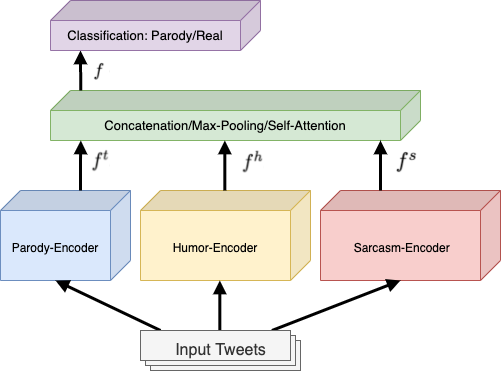
\includegraphics[width=5.5cm]{Model-Diagram_modified.png}
\caption{The structure of our \emph{multi-encoder} model for combining humor and sarcasm information for political parody prediction.}
\label{fig:model}
\end{figure}





\subsection{Text Encoders}
%Given a post  $T$, we first compute parody, humor, and sarcasm representations $f^t$, $f^h$, $f^s$ respectively.

\paragraph{Parody}

As a task-specific parody encoder, we use the vanilla pretrained BERTweet \citep{nguyen-etal-2020-bertweet}, a BERT \cite{devlin-etal-2019-bert} based model pre-trained on a corpus of English Tweets and fine-tuned on the parody data set (\S \ref{sec:data}). %%%We compute a contextual representation $f^p \in \mathbf{R}^{768}$ of $T$ by extracting the `classification' [CLS] token. 




\paragraph{Humor} 
To capture humor specific characteristics in social media text, we use the data set introduced by \citet{annamoradnejad2020colbert} which contains humorous and non-humorous short texts collected from Reddit and Huffington Post. First, we adapt BERTweet using domain-adaptive pre-training \citep{sun2020finetune,gururangan-etal-2020-dont} on 10,000 randomly selected humor-only short texts with masked language modeling. 
Subsequently, we use a continual learning strategy \citep{8107520,Sun_Wang_Li_Feng_Tian_Wu_Wang_2020} to gradually learn humor-specific properties by further fine-tuning BERTweet on a humor classification task (i.e., predicting whether a text is humorous or not) by using 40,000 randomly selected humorous and non-humorous short texts from the humor corpus described above (see Figure~\ref{fig:humorEncoder}).
%Finally, we obtain a humor representation $f^h \in \mathbf{R}^{768}$ of the input text by extracting the [CLS] token from our humor-adapted BERTweet model.




\begin{figure}[t!]
\centering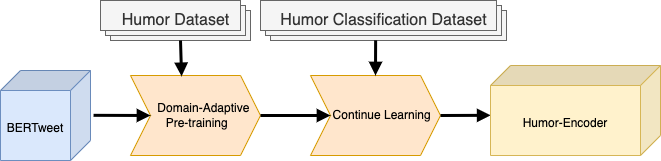
\includegraphics[width=7.5cm]{humor_encoder.png}
\caption{\textit{Humor Encoder}.}
\label{fig:humorEncoder}
\end{figure}

\begin{figure}[t!]
\centering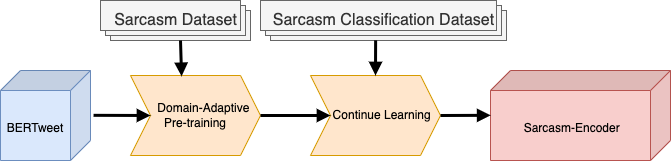
\includegraphics[width=7.5cm]{sarcasm_encoder.png}
\caption{\textit{Sarcasm Encoder}.}
\label{fig:sarcasmEncoder}
\end{figure}



\paragraph{Sarcasm} 
Similar to humor, we extract sarcasm-related semantic information from a post $T$ by using sarcasm annotated data sets from \citet{oprea-magdy-2020-isarcasm} and \citet{Rajadesingan2015SarcasmDO}. The first data set consists of 777 and 3,707 sarcasm and non-sarcasm posts from Twitter and the second data set consists of 9,104 sarcasm and more than 90,000 non-sarcasm posts from Twitter. We first perform domain-adaptive pre-training of BERTweet on all sarcastic posts with masked language modeling. Then, we fine-tune the model on a sarcasm classification task, similar to the humor encoder (see Figure~\ref{fig:sarcasmEncoder}). For the fine-tuning step, we use the 9,881 sarcastic tweets and 10,000 randomly sampled non-sarcasm tweets from the two data sets (i.e., 3,707 from the first and 6,293 from the second).

%Finally, the sarcasm text representation $f^s \in \mathbf{R}^{768}$ is obtained by extracting the [CLS] token from the sarcasm-adapted BERTweet.

%For adapting BERTweet on sarcasm, we select two data sets introduced by \citet{oprea-magdy-2020-isarcasm} and \citet{Rajadesingan2015SarcasmDO} respectively. The first data set consists of $777$ and $3707$ sarcasm and non-sarcasm posts from Twitter. The second data set consists of $9,104$ sarcasm and more than $90,000$ non-sarcasm posts from Twitter. For adaptive pre-training, we use all $9,881$ sarcasm tweets from both data sets ($777$ and $9,104$ respectively). We pretrain using a batch-size of $16$ over $5$ epochs with a learning rate of $2e^{-5}$. For fine-tuning on a sarcasm classification task, we use the $9,881$ sarcasm tweets and $10,000$ randomly sampled non-sarcasm tweets from the two data sets (i.e. $3,707$ from the first and $6,293$ from the second) using the same hyperparameters to the humor-specific encoder.


We compute parody $f^t$, humor $f^h$, and sarcasm $f^s$ representations by extracting the `classification' [CLS] token from each encoder respectively, where $f \in \mathbf{R}^{768}$.

%For adapting BERTweet on sarcasm, we use two data sets introduced by \citet{oprea-magdy-2020-isarcasm} and \citet{Rajadesingan2015SarcasmDO} respectively. The first data set consists of $777$ and $3707$ sarcasm and non-sarcasm posts from Twitter. The second data set consists of $9,104$ sarcasm and more than $90,000$ non-sarcasm posts from Twitter. For adaptive pre-training, we use all $9,881$ sarcasm tweets from both data sets ($777$ and $9,104$ respectively). %

%\paragraph{Further pretraining}
%In-Domain Further-Pretraining strategy also known as domain-adaptive pretraining \citep{sun2020finetune,gururangan-etal-2020-dont} provides a way to learn domain-specific data distribution by pretraining on specific data. Since the aim is to enhance our model with domain-specific semantics, we use masked-language modelling (MLM) as the pretraining task \citep{devlin-etal-2019-bert,liu2019roberta} for our experiments.

%\paragraph{continual learning}
%Continue Learning strategy \citep{8107520,Sun_Wang_Li_Feng_Tian_Wu_Wang_2020}, allows models to gradually learn domain-specific properties for certain task by training on independently supportive tasks.


\subsection{Combining Encoders}

We explore three approaches to combine $f^t$, $f^h$, and $f^s$ representations.

\paragraph{Concatenation} First, the three text representations are simply concatenated to form a combined representation $f \in \mathbf{R}^{768\times3}$. 


\paragraph{Self-Attention} We also use a 4-head self-attention\footnote{Early experimentation with larger attention heads did not improve results in the dev set.} mechanism \cite{NIPS2017_3f5ee243} on $f^t, f^h, f^s$. The goal is to find correlations between representations and learn the contribution of each encoder in the final representation. %The multi-semantic representation $f \in \mathbf{R}^{768}$ corresponds to the output of the general encoder $O^t$.% We use $O^t$ as the . %According to \citet{NIPS2017_3f5ee243},  self-attention will force the extracted text features from different semantic encoders to find the correlated information between each other and the Multi-head mechanism enables the found information is from different representation subspaces at different positions.

\paragraph{Max-Pooling} Finally, we perform a max-pooling operation on each dimension of $f^t$, $f^h$, $f^s$ to obtain a representation $f \in \mathbf{R}^{768}$. The aim is to use the most dominant features learned by each encoder. %(e.g. humor, sarcasm or parody). 

\subsection{Classification}
Finally, we pass the combined representation $f$ to a classification layer with a sigmoid activation function for predicting whether a post is a parody or not. Three encoders are fine-tuned simultaneously on the parody data set (\S \ref{sec:data}).\footnote{Early experimentation with humor and sarcasm encoders frozen during the fine-tuning process did not show any performance improvement.}

%Our humor encoder is domain- adaptive pretrained on corpus from other source, not twitter. Also, encoders may need some steps to learn vocabulary distributions in Parody tweet data sets.

\section{Experimental Setup}






\subsection{Data}
\label{sec:data}

We use the data set introduced by \citet{maronikolakis-etal-2020-analyzing} which contains 131,666 tweets written in English, with 65,956 tweets from political parody accounts and 65,710 tweets posted by real politician accounts. The data set is publicly available\footnote{\url{https://archive.org/details/parody_data_acl20}} and allows us to compare our results to state-of-the-art parody detection methods.  

We use the three data splits provided: (i) \emph{Person Split}, each split (train, dev, test) contains tweets from different real -- \emph{parody} account pairs; (ii) \emph{Gender Split}, two different splits based on the gender of the politicians (i.e., female accounts in train/dev and male in test, and male accounts in train/dev and female in test); \emph{Location Split}, data is split according to the location of the politicians in three groups (US, UK, Rest of the World or RoW). Each group is assigned to the test set and the other two groups to the train and dev sets.




\subsection{Baselines} 
%Implementation details for all models including humor and sarcasm encoders are included in Appendix \ref{appendix_details}. 

We compare our \emph{multi-encoder} models with %{\bf FastText} \cite{bojanowski-etal-2017-enriching} and 
transformers for parody detection \citep{maronikolakis-etal-2020-analyzing}: {\bf BERT} \citep{devlin-etal-2019-bert} and {\bf RoBERTa} \citep{liu2019roberta}. Also, we compare our models to {\bf BERTweet} \citep{nguyen-etal-2020-bertweet}. 

\subsection{Implementation details}
\label{imp_details}

\paragraph{Humor Encoder} 
For adaptive pre-training, the batch-size is set to $16$ and the number of training epochs is set to $3$ with a learning rate of $2e^{-5}$. For humor classification, we use batch size of $128$ and the number of epochs is set to $2$ with a learning rate of $3e^{-5}$.

\paragraph{Sarcasm Encoder} 
We pretrain using a batch-size of $16$ over $5$ epochs with a learning rate of $2e^{-5}$. For fine-tuning on a sarcasm classification task, we use the $9,881$ sarcasm tweets and $10,000$ randomly sampled non-sarcasm tweets from the two data sets (i.e., $3,707$ from the first and $6,293$ from the second) using the same hyperparameters to the humor-specific encoder.

\paragraph{Multi-encoder}
For the complete \emph{multi-encoder} model, we use a batch size of $128$ and the learning rate is set to $2e^{-5}$. The entire model is fine-tuned for $2$ epochs.%\footnote{In early experimentation, freezing the humor and sarcasm encoders resulted in lower performance in the dev set.} %The warm-up ratio for the cosine scheduler is $0.06$.

\subsection{Evaluation} 
We evaluate the performance of all models using F1 score as \citet{maronikolakis-etal-2020-analyzing}. Results are obtained over $3$ runs using different random seeds reporting average and standard deviation. 

%%%%%%%%%%%%%%%%%%%%%%%%%%%%%%%%%%%%%%%%%%%%%%%%%%%%%%%%%%%%%%%%%

\section{Results}
\label{sec:results}

\subsection{Predictive Performance}
%\paragraph{Single-Encoder}
Table \ref{tab:person} shows the results for parody detection on the \emph{Person Split}. %In general we observe that all transformer-based models (\textit{BERT}, \textit{RoBERTa}, \textit{BERTweet}) perform better than FastText (F1: $76.62$), which demonstrates the benefits of pre-trained contextual representations for parody detection. Among them, 
We observe that \textit{BERTweet} has the best performance (F1: $90.72$) among transformer-based models (\textit{BERT}, \textit{RoBERTa}, \textit{BERTweet}), outperforming previous state-of-the-art by \citet{maronikolakis-etal-2020-analyzing}. This is due to the fact that \textit{BERTweet} has been specifically pre-trained on Twitter text. Similar behavior is observed on the \emph{Gender} and \emph{Location} splits (see Table~\ref{tab:gender} and \ref{tab:location} respectively). %which confirms the superiority of \textit{BERTweet}.


\renewcommand{\arraystretch}{1.1}
\begin{table}[!t]
\small
\centering

%\resizebox{\linewidth}{!}{
\begin{tabular}{|l| c|}
\rowcolor[gray]{.7}\multicolumn{2}{|c|}{\textbf{Person}} \\\hline
\rowcolor[gray]{.7}\multicolumn{1}{|c|}{\textbf{Model}}& \multicolumn{1}{|c|}{\textbf{F1}} %& \multicolumn{1}{c}{\textbf{AUC}}
\\ \hline
\rowcolor[gray]{0.9}\multicolumn{2}{|l|}{\textbf{Single-Encoder}}\\
%\cellcolor[gray]{1}FastText & $76.62\pm1.21$ %& $76.62\pm2.13$
%\\
%\cellcolor[gray]{.97}BERT &  $90.49\pm0.39$ %& $90.39\pm0.42$
%\\
\cellcolor[gray]{1}BERT$^{\ast\ast}$ &  $87.65\pm0.18$ %& $90.39\pm0.42$
\\
%\cellcolor[gray]{.95}RoBERTa &  $88.77\pm0.33$ %& $88.76\pm0.36$
%\\
\cellcolor[gray]{1}RoBERTa$^{\ast\ast}$ & $89.66\pm0.33$ %& $\textbf{90.05}\pm\textbf{0.29}$
\\ 
\cellcolor[gray]{1}BERTweet & $90.72\pm0.31$ %& $\textbf{90.67}\pm\textbf{0.32}$
\\\hline
\rowcolor[gray]{0.9} \multicolumn{2}{|l|}{\textbf{Multi-encoder (Ours)}}\\
\cellcolor[gray]{1}Concatenation & $88.99\pm0.17$ %& $89.00\pm0.17$
\\ 
\cellcolor[gray]{1}Self-Attention & $\textbf{91.19} \pm\textbf{0.31}$ %& $\textbf{91.20}\pm\textbf{0.24}$
\\ 
\cellcolor[gray]{1}Max-Pooling & $91.05\pm0.30$% & $90.95\pm0.28$
\\ \hline
\end{tabular}
%}
\caption{F1-scores for parody detection on the \emph{Person Split}. $^{\ast\ast}$ Results from \citet{maronikolakis-etal-2020-analyzing}. %$\dagger$ indicates statistically significant improvement  over \textit{RoBERTa} (t-test, $p<0.05$). %Also, our best model achieves statistically significant improvement over BERTweet (t-test, $p < 0.05$) on gender splits.
Best results are in bold.}
\label{tab:person}
\end{table}



\begin{table}[!t]
\renewcommand{\arraystretch}{1.1}
\centering
\small
%\resizebox{\linewidth}{!}{
\begin{tabular}{ |l| c|c|}
\hline
\rowcolor[gray]{.7}\multicolumn{3}{|c|}{\textbf{Gender}} \\\hline
\rowcolor[gray]{.7}\multicolumn{1}{|c|}{\textbf{Model}} & \textbf{M$\to$F} & \textbf{F$\to$M} \\ \hline
\rowcolor[gray]{0.9} \multicolumn{3}{|l|}{\textbf{Single-Encoder}}\\
%\cellcolor[gray]{1}FastText & $77.74\pm2.01$ & $74.51\pm2.87$\\
%\cellcolor[gray]{.9}BERT & $87.43$ & $84.39$\\
\cellcolor[gray]{1}BERT$^{\ast\ast}$ & $85.85\pm0.28$ & $84.40\pm0.35$\\
%\cellcolor[gray]{.9}RoBERTa & $85.29$ & $84.10$\\
\cellcolor[gray]{1}RoBERTa$^{\ast\ast}$ & $87.11\pm0.31$ & $84.87\pm0.38$\\
\cellcolor[gray]{1}BERTweet & $88.01\pm0.29$ &  $85.57\pm0.27$\\ \hline
\rowcolor[gray]{0.9}\multicolumn{3}{|l|}{\textbf{Multi-encoder (Ours)}}  \\
\cellcolor[gray]{1}Concatenation & $86.84\pm0.15$ & $84.21\pm0.22$\\
\cellcolor[gray]{1}Self-Attention & $\textbf{89.97}\pm\textbf{0.34}$ & $\textbf{88.56}\pm\textbf{0.39}$\\ 
\cellcolor[gray]{1}Max-Pooling & $88.39\pm0.27$ & $86.89\pm0.56$\\ \hline

\end{tabular}
%}
\caption{F1-scores on the \emph{Gender Split}. %$\dagger$ denotes statistical significant improvement over BERTweet (t-test, $p<0.05$). 
$^{\ast\ast}$ Results from \citet{maronikolakis-etal-2020-analyzing}. Best results are in bold.}
\label{tab:gender}
\end{table}

%\paragraph{Multi-Semantics-Encoder}
Our proposed \emph{multi-encoder} achieves the best performance when using \textit{Self-Attention} to combine the three parallel encoders (F1: $91.19$; $89.97$, $88.56$; $88.37$, $87.91$, $87.16$; for \emph{Person}, \emph{Gender}, and \emph{Location} splits respectively). Moreover, it outperforms the best single-encoder model \textit{BERTweet} in the majority of cases which corroborates that parody detection benefits from combining general contextual representations with humor and sarcasm specific information, as humor and sarcasm are important characteristics of parody \citep{haiman1998talk,Parody_Humor}. On the other hand, simply concatenating the three parallel encoders degrades the performance across different splits (\emph{Person}: $88.99$; \emph{Gender}: $86.84$, $84.21$ \emph{Location}: $85.41$, $84.74$, $83.62$). This happens because the concatenation operation treats the three encoders as equally important. While humor and sarcasm are related to parody, they may not necessarily have the same relevance as indicators of parody. %Thus, in order to successfully combine different text representations, it is more desirable to extract the most relevant semantic information from each encoder rather than treating the tree encoders equally important.

%\textit{Max-Pooling} obtains comparable results to applying \textit{Self-Attention} (e.g. F1 for \emph{Person} is $91.05$) for all but the model that was trained on female accounts and tested on male accounts (F1: $86.89$). 
%In general, models trained on female accounts perform worse than those trained on male accounts which may be due to the unbalanced distribution of accounts across genders. However, o
Our best performing model (\textit{Self-Attention}) outperforms the vanilla \textit{BERTweet} by $3$ F1 points when trained on female accounts and by almost $2$ F1 points when trained on male accounts. We speculate that the additional linguistic information from the two encoders (i.e., sarcasm and humor) is more beneficial in low data settings. The number of female politicians is considerably smaller than males in the data set (see \citet{maronikolakis-etal-2020-analyzing} for more details). 


%Many male parody tweets tend to include cliché in their expression and these tweet’s parody-semantic intentions are more obscured. Comprehensive semantic (S+H+P) information is more needed to predict such tweets than highlighted partial semantics information. (This explains the performance gap between self-attention and max-pooling). 
%On the other hand, female parody tweets tends to include more obvious sarcastic or humorous trigger words. Their intention to express Parody (emphasizing humor or sarcasm) is more obvious. Female parody tweets serve like data augmentation for our model, which enables our Humor-Encoder and Sarcasm-Encoder to be more efficiently trained. (This explains why our model has a more obvious boost in F->M).



%%%%%%%%%%%%%%%%%%%%%%%%%%%%%%%%%%%%%%%%%%%%%%%%%%%%%%%%%%%%%%%%%




\renewcommand{\arraystretch}{1.1}
\begin{table}[!t]
\centering
\small
\resizebox{\linewidth}{!}{
\begin{tabular}{ |l|c|c|c|}
\hline
\rowcolor[gray]{.7}\multicolumn{4}{|c|}{\textbf{Location}}\\\hline
\rowcolor[gray]{.7}\multicolumn{1}{|c|}{\textbf{Model}} & \begin{tabular}{c}\textbf{UK+US}\\ \textbf{$\to$ RoW}\end{tabular}  & \begin{tabular}{c}\textbf{RoW+US} \\ \textbf{$\to$ UK} \end{tabular} 
& \begin{tabular}{c}\textbf{RoW+UK} \\ \textbf{$\to$ US}\end{tabular}\\ \hline 
\rowcolor[gray]{0.9} \multicolumn{4}{|l|}{\textbf{Single-Encoder}}\\
%\cellcolor[gray]{1}FastText & $77.62\pm1.53$ & $77.54\pm0.81$ & $76.18\pm2.24$\\ 
%\cellcolor[gray]{1}BERT & $87.73$ & $86.26$ & $84.51$\\ 
\cellcolor[gray]{1}BERT$^{\ast\ast}$ & $86.69\pm0.45$ & $83.78\pm0.19$ & $83.12\pm0.60$\\ 
%\cellcolor[gray]{1}RoBERTa & $86.92$ & $85.48$ & $84.79$\\
\cellcolor[gray]{1}RoBERTa$^{\ast\ast}$  & $87.70\pm0.45$ & $85.10\pm0.27$ & $85.99\pm0.61$\\
\cellcolor[gray]{1}BERTweet & $88.21\pm0.26$ & $87.85\pm0.24$ & $\textbf{87.18}\pm\textbf{0.41}$\\ \hline
\rowcolor[gray]{0.9} \multicolumn{4}{|l|}{\textbf{Multi-encoder (Ours)}}\\
\cellcolor[gray]{1}Concatenation & $85.41\pm0.26$ & $84.74\pm0.20$ & $83.62\pm0.35$\\ 
\cellcolor[gray]{1}Self-Attention & $\textbf{88.37}\pm\textbf{0.28}$ & $\textbf{87.91}\pm\textbf{0.19}$ & $87.16\pm0.37$\\ 
\cellcolor[gray]{1}Max-Pooling & $88.25\pm0.39$ & $86.49\pm0.33$ & $86.54\pm0.41$\\ \hline

\end{tabular}}
\caption{F1-scores on the \emph{Location Split}. %$\dagger$ denotes statistically significant improvement over BERTweet (t-test, $p<0.05$).
$^{\ast\ast}$ Results from \citet{maronikolakis-etal-2020-analyzing}. Best results are in bold.
}
\label{tab:location}
\end{table}



%%%%%%%%%%%% Ablation Study %%%%%%%%%%%%%%%%%
\subsection{Ablation Study} 
We also examine the effect of combining parody-specific representations with humor and sarcasm information by running an ablation study. We compare performance of four models: using parody representations only (P), and combining parody representations with humor (P+H), or sarcasm (P+S) information, as well as with both (P+S+H). The results of this analysis are depicted in Tables~\ref{tab:person_complete}, \ref{tab:gender_complete} and \ref{tab:location_complete}. We observe that both sarcasm and humor contribute to the performance gain, but using both is more beneficial. Modelling sarcasm leads to more gains than humor and this could be attributed to the characteristics of the parody corpus, namely that it focuses primarily on the political domain, which have a high sarcastic component \citep{anderson2017social}.

%%%%%%%%%%%%%%%%%%%%%%%%%%%%%%%%%%%%%%%%%%%%%%%%%%%%%%%%%%%%%%%%%
%\begin{table}[!t]
%\small
%\centering
%\begin{tabular}{|l| c|}
%\rowcolor[gray]{.7}\multicolumn{2}{|c|}{\textbf{Person}} %\\\hline
%\rowcolor[gray]{.7}\multicolumn{1}{|c|}{\textbf{Model}}& %\multicolumn{1}{|c|}{\textbf{F1}} %& %\multicolumn{1}{c}{\textbf{AUC}}
%\\ \hline
%\rowcolor[gray]{0.9}\multicolumn{2}{|l|}{\textbf{Single-Encoder}}\\
%\cellcolor[gray]{1}BERTweet (P) & $90.72\pm0.31$ 
%\\\hline
%\rowcolor[gray]{0.9} %\multicolumn{2}{|l|}{\textbf{Multi-encoder (Ours)}}\\
%\cellcolor[gray]{1}Self-Attention (P+H)& $90.98\pm0.36$ 
%\\
%\cellcolor[gray]{1}Self-Attention (P+S) & $91.14\pm0.40$ 
%\\ 
%\cellcolor[gray]{1}Self-Attention (P+S+H) & $\textbf{91.19} %\pm\textbf{0.31}$ 

%\\ \hline
%\end{tabular}
%\caption{Parody detection on the \emph{Person Split} using the \textit{Self-Attention} \emph{multi-encoder} with: parody (P) representations only, combining parody representations with humor (P+H), sarcasm (P+S), or both (P+S+H). %Best results are in bold.
%}
%\label{tab:person_ablation}
%\end{table}
%%%%%%%%%%%%%%%%%%%%%%%%%%%%%%%%%%%%%%%%%%%%%%%%%%%%%%%%%%%%%

% FULL ABLATION TABLES FROM APPX
\renewcommand{\arraystretch}{1.2}
\begin{table}[!h]
\small
\centering
%\resizebox{\linewidth}{!}{
\begin{tabular}{|l| c|}
\rowcolor[gray]{.7}\multicolumn{2}{|c|}{\textbf{Person}} \\\hline
\rowcolor[gray]{.7}\multicolumn{1}{|c|}{\textbf{Model}}& \multicolumn{1}{|c|}{\textbf{F1}} %& \multicolumn{1}{c}{\textbf{AUC}}
\\ \hline
\rowcolor[gray]{0.9}\multicolumn{2}{|l|}{\textbf{Single-Encoder}}\\
%\cellcolor[gray]{1}FastText & $76.62\pm1.21$ %& $76.62\pm2.13$
%\\
%\cellcolor[gray]{.97}BERT &  $90.49\pm0.39$ %& $90.39\pm0.42$
%\\
%\cellcolor[gray]{1}BERT$^{\ast\ast}$ &  $87.65\pm0.18$ %& $90.39\pm0.42$
%\\
%\cellcolor[gray]{.95}RoBERTa &  $88.77\pm0.33$ %& $88.76\pm0.36$
%\\
%\cellcolor[gray]{1}RoBERTa$^{\ast\ast}$ & $89.66\pm0.33$ %& $\textbf{90.05}\pm\textbf{0.29}$
%\\ 
\cellcolor[gray]{1}BERTweet (P) & $90.72\pm0.31$ %& $\textbf{90.67}\pm\textbf{0.32}$
\\\hline
\rowcolor[gray]{0.9} \multicolumn{2}{|l|}{\textbf{Multi-encoder (Ours)}}\\
\cellcolor[gray]{1}Concatenation (P+S+H) & $88.99\pm0.17$ %& $89.00\pm0.17$
\\ 
\cellcolor[gray]{1}Concatenation (P+S) & $90.51\pm0.26$ %& $89.00\pm0.17$
\\ 
\cellcolor[gray]{1}Concatenation (P+H) & $89.98\pm0.23$ %& $89.00\pm0.17$
\\ 
\cellcolor[gray]{1}Self-Attention (P+S+H) & $\textbf{91.19} \pm\textbf{0.31}$ %& $\textbf{91.20}\pm\textbf{0.24}$
\\ 
\cellcolor[gray]{1}Self-Attention (P+S) & $91.14\pm0.40$ %& $\textbf{91.20}\pm\textbf{0.24}$
\\ 
\cellcolor[gray]{1}Self-Attention (P+H)& $90.98\pm0.36$ %& $\textbf{91.20}\pm\textbf{0.24}$
\\ 
\cellcolor[gray]{1}Max-Pooling\hspace{0.44em} (P+S+H) & $91.05\pm0.30$% & $90.95\pm0.28$
\\ 
\cellcolor[gray]{1}Max-Pooling\hspace{0.44em} (P+S) & $91.06\pm0.39$% & $90.95\pm0.28$
\\ 
\cellcolor[gray]{1}Max-Pooling\hspace{0.44em} (P+H) & $90.78\pm0.42$% & $90.95\pm0.28$
\\ \hline
\end{tabular}
%}
\caption{F1-scores for parody detection on the \emph{Person Split} with various settings: parody (P) representations only, and combining parody representations with humor (P+H), or sarcasm (P+S) information, as well as with both (P+S+H). Best results are in bold.
}
\label{tab:person_complete}
\end{table}



\renewcommand{\arraystretch}{1.2}
\begin{table}[!t]
\centering
\small
%\resizebox{\linewidth}{!}{
\begin{tabular}{ |l| c|c|}
\hline
\rowcolor[gray]{.7}\multicolumn{3}{|c|}{\textbf{Gender}} \\\hline
\rowcolor[gray]{.7}\multicolumn{1}{|c|}{\textbf{Model}} & \textbf{M$\to$F} & \textbf{F$\to$M} \\ \hline
\rowcolor[gray]{0.9} \multicolumn{3}{|l|}{\textbf{Single-Encoder}}\\
\cellcolor[gray]{1}BERTweet (P) & $88.01\pm0.29$ &  $85.57\pm0.27$\\ \hline
%\cellcolor[gray]{1}FastText & $77.74\pm2.01$ & $74.51\pm2.87$\\
%\cellcolor[gray]{.9}BERT & $87.43$ & $84.39$\\
%\cellcolor[gray]{1}BERT$^{\ast\ast}$ & $85.85\pm0.28$ & $84.40\pm0.35$\\
%\cellcolor[gray]{1}RoBERTa$^{\ast\ast}$ & $87.11\pm0.31$ & $84.87\pm0.38$\\
\rowcolor[gray]{0.9}\multicolumn{3}{|l|}{\textbf{Multi-encoder (Ours)}}  \\
\cellcolor[gray]{1}Concatenation (P+S+H)& $86.84\pm0.15$ & $84.21\pm0.22$\\
\cellcolor[gray]{1}Concatenation (P+S)& $86.93\pm0.40$ & $83.70\pm0.41$\\
\cellcolor[gray]{1}Concatenation (P+H)& $86.58\pm0.31$ & $83.34\pm0.38$\\
\cellcolor[gray]{1}Self-Attention (P+S+H)& $\textbf{89.97}\pm\textbf{0.34}$ & $\textbf{88.56}\pm\textbf{0.39}$\\ 
\cellcolor[gray]{1}Self-Attention (P+S)& $89.49\pm0.37$ & $88.23\pm0.44$\\ 
\cellcolor[gray]{1}Self-Attention (P+H)& $88.71\pm0.42$ & $87.62\pm0.50$\\ 
\cellcolor[gray]{1}Max-Pooling\hspace{0.44em} (P+S+H)& $88.39\pm0.27$ & $86.89\pm0.56$\\ 
\cellcolor[gray]{1}Max-Pooling\hspace{0.44em} (P+S)& $88.36\pm0.46$ & $86.55\pm0.49$\\
\cellcolor[gray]{1}Max-Pooling\hspace{0.44em} (P+H)& $88.14\pm0.52$ & $86.53\pm0.53$\\\hline

\end{tabular}
%}
\caption{
F1-scores for parody detection on the \emph{Gender Split} with various settings: parody (P) representations only, and combining parody representations with humor (P+H), or sarcasm (P+S) information, as well as with both (P+S+H). Best results are in bold.}
\label{tab:gender_complete}
\end{table}

\renewcommand{\arraystretch}{1.2}
\begin{table}[!t]
\centering
\small
\resizebox{\linewidth}{!}{
\begin{tabular}{ |l|c|c|c|}
\hline
\rowcolor[gray]{.7}\multicolumn{4}{|c|}{\textbf{Location}}\\\hline
\rowcolor[gray]{.7}\multicolumn{1}{|c|}{\textbf{Model}} & \begin{tabular}{c}\textbf{UK+US}\\ \textbf{$\to$ RoW}\end{tabular}  & \begin{tabular}{c}\textbf{RoW+US} \\ \textbf{$\to$ UK} \end{tabular} 
& \begin{tabular}{c}\textbf{RoW+UK} \\ \textbf{$\to$ US}\end{tabular}\\ \hline 
\rowcolor[gray]{0.9} \multicolumn{4}{|l|}{\textbf{Single-Encoder}}\\
\cellcolor[gray]{1}BERTweet (P) & $88.21\pm0.26$ & $87.85\pm0.24$ & $\textbf{87.18}\pm\textbf{0.41}$\\ \hline

%\cellcolor[gray]{1}FastText & $77.62\pm1.53$ & $77.54\pm0.81$ & $76.18\pm2.24$\\ 
%\cellcolor[gray]{1}BERT & $87.73$ & $86.26$ & $84.51$\\ 
%\cellcolor[gray]{1}BERT$^{\ast\ast}$ & $86.69\pm0.45$ & $83.78\pm0.19$ & $83.12\pm0.60$\\ 
%\cellcolor[gray]{1}RoBERTa & $86.92$ & $85.48$ & $84.79$\\
%\cellcolor[gray]{1}RoBERTa$^{\ast\ast}$  & $87.70\pm0.45$ & $85.10\pm0.27$ & $85.99\pm0.61$\\

\rowcolor[gray]{0.9} \multicolumn{4}{|l|}{\textbf{Multi-encoder (Ours)}}\\
\cellcolor[gray]{1}Concatenation (P+S+H) & $85.41\pm0.26$ & $84.74\pm0.20$ & $83.62\pm0.35$\\
\cellcolor[gray]{1}Concatenation (P+S) & $85.92\pm0.24$ & $85.67\pm0.18$ & $84.09\pm0.39$\\
\cellcolor[gray]{1}Concatenation (P+H) & $85.39\pm0.29$ & $85.33\pm0.26$ & $83.75\pm0.44$\\
\cellcolor[gray]{1}Self-Attention (P+S+H) & $\textbf{88.37}\pm\textbf{0.28}$ & $\textbf{87.91}\pm\textbf{0.19}$ & $87.16\pm0.37$\\ 
\cellcolor[gray]{1}Self-Attention (P+S) & $88.24\pm0.33$ & $87.88\pm0.23$ & $86.47\pm0.32$\\
\cellcolor[gray]{1}Self-Attention (P+H) & $88.13\pm0.35$ & $87.05\pm0.28$ & $85.36\pm0.40$\\
\cellcolor[gray]{1}Max-Pooling\hspace{0.44em}  (P+S+H) & $88.25\pm0.39$ & $86.49\pm0.33$ & $86.54\pm0.41$\\
\cellcolor[gray]{1}Max-Pooling\hspace{0.44em} (P+S) & $88.28\pm0.42$ & $87.83\pm0.39$ & $86.56\pm0.36$\\
\cellcolor[gray]{1}Max-Pooling\hspace{0.44em} (P+H) & $88.22\pm0.52$ & $86.44\pm0.42$ & $85.96\pm0.45$\\
\hline

\end{tabular}
}
\caption{
F1-scores for parody detection on the \emph{Location Split} with various settings: parody (P) representations only, and combining parody representations with humor (P+H), or sarcasm (P+S) information, as well as with both (P+S+H). Best results are in bold.}
\label{tab:location_complete}
\end{table}
%%%%%%%%%%%%%%%%%%%%%%%%%%%%%%%%%%%%%%%%%%%%%%%%%%%%%%%%%%%%%
\section{Error Analysis}

Finally, we perform an error analysis to examine the behavior and limitations of our best-performing model (\emph{multi-encoder} with Self-Attention). 

The next two examples correspond to real tweets that were misclassified as parody:
\begin{itemize}
%The first example comes from the user @tedwheeler and his tweet is listed below:  
%\begin{quotation}
%@EvertonBailey!
\item [(1)]  \textit{Congratulations, <mention>! <url>.}
%\end{quotation}
%\begin{quotation}
%The second example comes from the user @Jeremy\_Hunt and his tweet is listed below:
\item [(2)] \textit{It's a shame that Boris isn't here answering questions from the public this evening.}
%\end{quotation}
\end{itemize}
We speculate that the model misclassified these tweets as parody because they contain terms that are related to sarcastic short texts such as user mentions, punctuation marks (\textit{!}), and negation (\textit{isn't}) \cite{gonzalez-ibanez-etal-2011-identifying,Parody_Humor}.


The following two examples correspond to parody tweets that were misclassified as real:
\begin{itemize}
%The first example comes from the user @InvisibleObama and his tweet is listed below:
%\begin{quotation}
\item [(3)] \textit{Hey America, it’s time to use your safe word.}
%\end{quotation}
%The second example comes from the user @Vestager\_EU and his tweet is listed below:
%\begin{quotation}
\item [(4)]\textit{I fully support the Digital Singles Market.}
%\end{quotation}
\end{itemize}

Example (3) is a call-to-action message, while Example (4) is a statement expressing support for a particular subject. These statements are written in a style that is similar to political slogans or campaign speeches \citep{fowler2021political} that the model fails to recognise. As a result, in addition to humor and sarcasm semantics, the model might be improved by integrating knowledge from the political domain such as from political speeches.


\section{Conclusion}

In this paper, we studied the impact of jointly modelling figurative devices to improve predictive performance of political parody detection in tweets. Our motivation was based on  studies in linguistics which emphasize the humorous and sarcastic components of parody \citep{haiman1998talk,Parody_Humor}. We presented a method that combines parallel encoders to capture parody, humor, and sarcasm specific representations from input sequences, which outperforms previous state-of-the-art proposed by \citet{maronikolakis-etal-2020-analyzing}. %Finally, we presented a thorough analysis of the shortcomings of current state-of-the-art models to distinguishing nuances in figurative language. 

In the future, we plan to combine information from other modalities (e.g., images) for improving parody detection~\citep{sanchez-villegas-aletras-2021-point,sanchez-villegas-etal-2021-analyzing}.


\section*{Acknowledgements}
We would like to thank all reviewers for their valuable feedback. DSV is supported by the Centre for Doctoral Training in Speech and Language Technologies (SLT) and their Applications funded by the
UK Research and Innovation grant EP/S023062/1.

\bibliography{anthology,custom}
\bibliographystyle{acl_natbib}

\appendix
\clearpage
% \section{Humor and Sarcasm Encoders}
% \label{sec:appendix_encoders}

% Fig. \ref{fig:sarcasmEncoder}. and Fig. \ref{fig:humorEncoder} show the structure of our sarcasm encoder and the humor encoder respectively explained in Section \ref{sec:model}.

% \begin{figure}[h!]
% \centering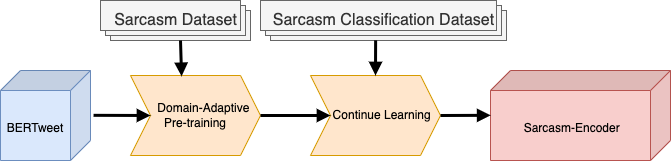
\includegraphics[width=7.5cm]{sarcasm_encoder.png}
% \caption{The structure of our \textit{Sarcasm Encoder}.}
% \label{fig:sarcasmEncoder}
% \end{figure}


% \begin{figure}[h!]
% \centering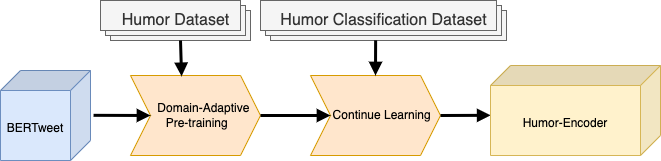
\includegraphics[width=7.5cm]{humor_encoder.png}
% \caption{The structure of our \textit{Humor Encoder}.}
% \label{fig:humorEncoder}
% \end{figure}


%\subsection{Implementation details}
%\label{appendix_details}
%%The implementation details for different parts of our model is listed as follows.
%\paragraph{Humor Encoder} 
%%For adaptive pre-training and humor specific fine-tuning, we use the data set introduced by \citet{annamoradnejad2020colbert} that contains humorous and non-humorous short texts from Reddit and Huffington Post. We split the data in: (1) $10,000$ randomly selected humor-only texts for adaptive pre-training; and (2) $40,000$ randomly selected humorous and non-humorous texts for task-specific fine-tuning (e.g. predicting whether a text is humorous or not). 
%For adaptive pre-training, the batch-size is set to $16$ and the number of training epochs is set to $3$ with a learning rate of $2e^{-5}$. For humor classification, we use batch size of $128$ and the number of epochs is set to $2$ with a learning rate of $3e^{-5}$.

%\paragraph{Sarcasm Encoder} 

%%For adapting BERTweet on sarcasm, we use two data sets introduced by \citet{oprea-magdy-2020-isarcasm} and \citet{Rajadesingan2015SarcasmDO} respectively. The first data set consists of $777$ and $3707$ sarcasm and non-sarcasm posts from Twitter. The second data set consists of $9,104$ sarcasm and more than $90,000$ non-sarcasm posts from Twitter. For adaptive pre-training, we use all $9,881$ sarcasm tweets from both data sets ($777$ and $9,104$ respectively). %
%We pretrain using a batch-size of $16$ over $5$ epochs with a learning rate of $2e^{-5}$. For fine-tuning on a sarcasm classification task, we use the $9,881$ sarcasm tweets and $10,000$ randomly sampled non-sarcasm tweets from the two data sets (i.e., $3,707$ from the first and $6,293$ from the second) using the same hyperparameters to the humor-specific encoder.

%\paragraph{Multi-encoder}
%For the complete \emph{multi-encoder} model, we use a batch size of $128$ and the learning rate is set to $2e^{-5}$. The entire model is fine-tuned for $2$ epochs.\footnote{In early experimentation, freezing the humor and sarcasm encoders resulted in lower performance in the dev set.} %The warm-up ratio for the cosine scheduler is $0.06$.




% \section{Implementation details}
% \label{appendix_details}
% %The implementation details for different parts of our model is listed as follows.
% \paragraph{Humor Encoder} 
% For adaptive pre-training and humor specific fine-tuning, we use the data set introduced by \citet{annamoradnejad2020colbert}. It contains humorous and non-humorous short texts collected from Reddit and Huffington Post. We split the data into two collections: (1) $10,000$ randomly selected humor-only short texts for adaptive pre-training; and (2) $40,000$ randomly selected humorous and non-humorous short texts for task-specific fine-tuning (e.g. predicting whether a text is humorous or not). For adaptive pre-training, the batch-size is set to $16$ and the number of training epochs is set to $3$ with a learning rate of $2e^{-5}$. For humor classification, we use batch size of $128$ and the number of epochs is set to $2$ with a learning rate of $3e^{-5}$.

% \paragraph{Sarcasm Encoder} 

% For adapting BERTweet on sarcasm, we select two data sets introduced by \citet{oprea-magdy-2020-isarcasm} and \citet{Rajadesingan2015SarcasmDO} respectively. The first data set consists of $777$ and $3707$ sarcasm and non-sarcasm posts from Twitter. The second data set consists of $9,104$ sarcasm and more than $90,000$ non-sarcasm posts from Twitter. For adaptive pre-training, we use all $9,881$ sarcasm tweets from both data sets ($777$ and $9,104$ respectively). We pretrain using a batch-size of $16$ over $5$ epochs with a learning rate of $2e^{-5}$. For fine-tuning on a sarcasm classification task, we use the $9,881$ sarcasm tweets and $10,000$ randomly sampled non-sarcasm tweets from the two data sets (i.e., $3,707$ from the first and $6,293$ from the second) using the same hyperparameters to the humor-specific encoder.

% \paragraph{Multi-encoder}
% For the complete \emph{multi-encoder} model, we use a batch size of $128$ and the learning rate is set to $2e^{-5}$. The entire model is fine-tuned for $2$ epochs.\footnote{In early experimentation, freezing the humor and sarcasm encoders resulted in lower performance in the dev set.} %The warm-up ratio for the cosine scheduler is $0.06$.


% \section{Ablation Study}
% \label{appendix_ablation}

% To examine the effect of combining parody-specific representations with humor and sarcasm information separately, we compare our models using parody representations only (P), and combining parody representations with humor (P+H), or sarcasm (P+S) information, as well as with both (P+S+H). The results of this analysis are depicted in Tables~\ref{tab:person_complete}, \ref{tab:gender_complete} and \ref{tab:location_complete}, and analysis is included in Section \ref{sec:results}.

%During the process to construct our model, we also tested several variant encoder combinations. The complete results are listed in Table~\ref{tab:person_complete},\ref{tab:gender_complete} and \ref{tab:location_complete}. Generally, the model consisting of Parody and Sarcasm encoder outperforms the model consisting of Parody and Humor encoders. Even, in some minority cases, the model consisting of Parody and Sarcasm encoder outperforms the model using all three encoders. This phenomenon further proves that the domain and source of a corpus will impact the performance of a pertained model. Unlike Sarcasm Encoder, our  Humor Encoder is domain-adaptive pre-trained and continually learned on corpus other than tweets data set. In addition, our test tweet data set is in mainly on political topics, which will have more emphasize on sarcasm semantics than humorous ones \citep{Parody_Sarcasm}.




% \begin{table}[!t]
% \small
% \centering

% %\resizebox{\linewidth}{!}{
% \begin{tabular}{|l| c|}
% \rowcolor[gray]{.7}\multicolumn{2}{|c|}{\textbf{Person}} \\\hline
% \rowcolor[gray]{.7}\multicolumn{1}{|c|}{\textbf{Model}}& \multicolumn{1}{|c|}{\textbf{F1}} %& \multicolumn{1}{c}{\textbf{AUC}}
% \\ \hline
% \rowcolor[gray]{0.9}\multicolumn{2}{|l|}{\textbf{Single-Encoder}}\\
% %\cellcolor[gray]{1}FastText & $76.62\pm1.21$ %& $76.62\pm2.13$
% %\\
% %\cellcolor[gray]{.97}BERT &  $90.49\pm0.39$ %& $90.39\pm0.42$
% %\\
% %\cellcolor[gray]{1}BERT$^{\ast\ast}$ &  $87.65\pm0.18$ %& $90.39\pm0.42$
% %\\
% %\cellcolor[gray]{.95}RoBERTa &  $88.77\pm0.33$ %& $88.76\pm0.36$
% %\\
% %\cellcolor[gray]{1}RoBERTa$^{\ast\ast}$ & $89.66\pm0.33$ %& $\textbf{90.05}\pm\textbf{0.29}$
% %\\ 
% \cellcolor[gray]{1}BERTweet (P) & $90.72\pm0.31$ %& $\textbf{90.67}\pm\textbf{0.32}$
% \\\hline
% \rowcolor[gray]{0.9} \multicolumn{2}{|l|}{\textbf{Multi-encoder (Ours)}}\\
% \cellcolor[gray]{1}Concatenation (P+S+H) & $88.99\pm0.17$ %& $89.00\pm0.17$
% \\ 
% \cellcolor[gray]{1}Concatenation (P+S) & $90.51\pm0.26$ %& $89.00\pm0.17$
% \\ 
% \cellcolor[gray]{1}Concatenation (P+H) & $89.98\pm0.23$ %& $89.00\pm0.17$
% \\ 
% \cellcolor[gray]{1}Self-Attention (P+S+H) & $\textbf{91.19} \pm\textbf{0.31}$ %& $\textbf{91.20}\pm\textbf{0.24}$
% \\ 
% \cellcolor[gray]{1}Self-Attention (P+S) & $91.14\pm0.40$ %& $\textbf{91.20}\pm\textbf{0.24}$
% \\ 
% \cellcolor[gray]{1}Self-Attention (P+H)& $90.98\pm0.36$ %& $\textbf{91.20}\pm\textbf{0.24}$
% \\ 
% \cellcolor[gray]{1}Max-Pooling\hspace{0.44em} (P+S+H) & $91.05\pm0.30$% & $90.95\pm0.28$
% \\ 
% \cellcolor[gray]{1}Max-Pooling\hspace{0.44em} (P+S) & $91.06\pm0.39$% & $90.95\pm0.28$
% \\ 
% \cellcolor[gray]{1}Max-Pooling\hspace{0.44em} (P+H) & $90.78\pm0.42$% & $90.95\pm0.28$
% \\ \hline
% \end{tabular}
% %}
% \caption{F1-scores for parody detection on the \emph{Person Split} with various settings: parody (P) representations only, and combining parody representations with humor (P+H), or sarcasm (P+S) information, as well as with both (P+S+H). Best results are in bold.
% }
% \label{tab:person_complete}
% \end{table}




% \begin{table}[!t]
% \renewcommand{\arraystretch}{1.1}
% \centering
% \small
% %\resizebox{\linewidth}{!}{
% \begin{tabular}{ |l| c|c|}
% \hline
% \rowcolor[gray]{.7}\multicolumn{3}{|c|}{\textbf{Gender}} \\\hline
% \rowcolor[gray]{.7}\multicolumn{1}{|c|}{\textbf{Model}} & \textbf{M$\to$F} & \textbf{F$\to$M} \\ \hline
% \rowcolor[gray]{0.9} \multicolumn{3}{|l|}{\textbf{Single-Encoder}}\\
% \cellcolor[gray]{1}BERTweet (P) & $88.01\pm0.29$ &  $85.57\pm0.27$\\ \hline
% %\cellcolor[gray]{1}FastText & $77.74\pm2.01$ & $74.51\pm2.87$\\
% %\cellcolor[gray]{.9}BERT & $87.43$ & $84.39$\\
% %\cellcolor[gray]{1}BERT$^{\ast\ast}$ & $85.85\pm0.28$ & $84.40\pm0.35$\\
% %\cellcolor[gray]{1}RoBERTa$^{\ast\ast}$ & $87.11\pm0.31$ & $84.87\pm0.38$\\
% \rowcolor[gray]{0.9}\multicolumn{3}{|l|}{\textbf{Multi-encoder (Ours)}}  \\
% \cellcolor[gray]{1}Concatenation (P+S+H)& $86.84\pm0.15$ & $84.21\pm0.22$\\
% \cellcolor[gray]{1}Concatenation (P+S)& $86.93\pm0.40$ & $83.70\pm0.41$\\
% \cellcolor[gray]{1}Concatenation (P+H)& $86.58\pm0.31$ & $83.34\pm0.38$\\
% \cellcolor[gray]{1}Self-Attention (P+S+H)& $\textbf{89.97}\pm\textbf{0.34}$ & $\textbf{88.56}\pm\textbf{0.39}$\\ 
% \cellcolor[gray]{1}Self-Attention (P+S)& $89.49\pm0.37$ & $88.23\pm0.44$\\ 
% \cellcolor[gray]{1}Self-Attention (P+H)& $88.71\pm0.42$ & $87.62\pm0.50$\\ 
% \cellcolor[gray]{1}Max-Pooling\hspace{0.44em} (P+S+H)& $88.39\pm0.27$ & $86.89\pm0.56$\\ 
% \cellcolor[gray]{1}Max-Pooling\hspace{0.44em} (P+S)& $88.36\pm0.46$ & $86.55\pm0.49$\\
% \cellcolor[gray]{1}Max-Pooling\hspace{0.44em} (P+H)& $88.14\pm0.52$ & $86.53\pm0.53$\\\hline

% \end{tabular}
% %}
% \caption{
% F1-scores for parody detection on the \emph{Gender Split} with various settings: parody (P) representations only, and combining parody representations with humor (P+H), or sarcasm (P+S) information, as well as with both (P+S+H). Best results are in bold.}
% \label{tab:gender_complete}
% \end{table}


% \begin{table}[!t]
% \centering
% \small
% \resizebox{\linewidth}{!}{
% \begin{tabular}{ |l|c|c|c|}
% \hline
% \rowcolor[gray]{.7}\multicolumn{4}{|c|}{\textbf{Location}}\\\hline
% \rowcolor[gray]{.7}\multicolumn{1}{|c|}{\textbf{Model}} & \begin{tabular}{c}\textbf{UK+US}\\ \textbf{$\to$ RoW}\end{tabular}  & \begin{tabular}{c}\textbf{RoW+US} \\ \textbf{$\to$ UK} \end{tabular} 
% & \begin{tabular}{c}\textbf{RoW+UK} \\ \textbf{$\to$ US}\end{tabular}\\ \hline 
% \rowcolor[gray]{0.9} \multicolumn{4}{|l|}{\textbf{Single-Encoder}}\\
% \cellcolor[gray]{1}BERTweet (P) & $88.21\pm0.26$ & $87.85\pm0.24$ & $\textbf{87.18}\pm\textbf{0.41}$\\ \hline

% %\cellcolor[gray]{1}FastText & $77.62\pm1.53$ & $77.54\pm0.81$ & $76.18\pm2.24$\\ 
% %\cellcolor[gray]{1}BERT & $87.73$ & $86.26$ & $84.51$\\ 
% %\cellcolor[gray]{1}BERT$^{\ast\ast}$ & $86.69\pm0.45$ & $83.78\pm0.19$ & $83.12\pm0.60$\\ 
% %\cellcolor[gray]{1}RoBERTa & $86.92$ & $85.48$ & $84.79$\\
% %\cellcolor[gray]{1}RoBERTa$^{\ast\ast}$  & $87.70\pm0.45$ & $85.10\pm0.27$ & $85.99\pm0.61$\\

% \rowcolor[gray]{0.9} \multicolumn{4}{|l|}{\textbf{Multi-encoder (Ours)}}\\
% \cellcolor[gray]{1}Concatenation (P+S+H) & $85.41\pm0.26$ & $84.74\pm0.20$ & $83.62\pm0.35$\\
% \cellcolor[gray]{1}Concatenation (P+S) & $85.92\pm0.24$ & $85.67\pm0.18$ & $84.09\pm0.39$\\
% \cellcolor[gray]{1}Concatenation (P+H) & $85.39\pm0.29$ & $85.33\pm0.26$ & $83.75\pm0.44$\\
% \cellcolor[gray]{1}Self-Attention (P+S+H) & $\textbf{88.37}\pm\textbf{0.28}$ & $\textbf{87.91}\pm\textbf{0.19}$ & $87.16\pm0.37$\\ 
% \cellcolor[gray]{1}Self-Attention (P+S) & $88.24\pm0.33$ & $87.88\pm0.23$ & $86.47\pm0.32$\\
% \cellcolor[gray]{1}Self-Attention (P+H) & $88.13\pm0.35$ & $87.05\pm0.28$ & $85.36\pm0.40$\\
% \cellcolor[gray]{1}Max-Pooling\hspace{0.44em}  (P+S+H) & $88.25\pm0.39$ & $86.49\pm0.33$ & $86.54\pm0.41$\\
% \cellcolor[gray]{1}Max-Pooling\hspace{0.44em} (P+S) & $88.28\pm0.42$ & $87.83\pm0.39$ & $86.56\pm0.36$\\
% \cellcolor[gray]{1}Max-Pooling\hspace{0.44em} (P+H) & $88.22\pm0.52$ & $86.44\pm0.42$ & $85.96\pm0.45$\\
% \hline

% \end{tabular}}
% \caption{
% F1-scores for parody detection on the \emph{Location Split} with various settings: parody (P) representations only, and combining parody representations with humor (P+H), or sarcasm (P+S) information, as well as with both (P+S+H). Best results are in bold.}
% \label{tab:location_complete}
% \end{table}

\section{Multitask-Learning}
\label{appendix_MTL}
We also tested applying \emph{multi-task learning} approaches \citep{Caruana93multitasklearning:} to use either sarcasm prediction (P+S), humor prediction (P+H) or both (P+S+H) as auxiliary tasks for parody detection. We utilize BERTweet as the share encoder and independent classification layers for parody and humor or sarcasm. %These independent layers are stacked. 
Three sets of weights are applied to losses from each independent classification layer and the three layers are stacked.
The best results are chosen and depicted in Table~\ref{tab:person_mtl}, Table \ref{tab:gender_mtl} and Table \ref{tab:location_mtl}.

\begin{table}[!h]
\small
\centering

%\resizebox{\linewidth}{!}{
\begin{tabular}{|l| c|}
\rowcolor[gray]{.7}\multicolumn{2}{|c|}{\textbf{Person}} \\\hline
\rowcolor[gray]{.7}\multicolumn{1}{|c|}{\textbf{Model}}& \multicolumn{1}{|c|}{\textbf{F1}} %& \multicolumn{1}{c}{\textbf{AUC}}
\\ \hline
%\cellcolor[gray]{1}FastText & $76.62\pm1.21$ %& $76.62\pm2.13$
%\\
%\cellcolor[gray]{.97}BERT &  $90.49\pm0.39$ %& $90.39\pm0.42$
%\\
\rowcolor[gray]{0.9}\multicolumn{2}{|l|}{\textbf{Single-Encoder}}\\
\cellcolor[gray]{1}BERTweet (P) & $\textbf{90.72}\pm\textbf{0.31}$ 
\\\hline
\rowcolor[gray]{0.9}\multicolumn{2}{|l|}{\textbf{Multi-Task}}\\
\cellcolor[gray]{1}P+S+H &  $87.46\pm0.18$ %& $90.39\pm0.42$
\\
\cellcolor[gray]{1}P+S & $89.41 \pm 0.31$ %& $\textbf{90.05}\pm\textbf{0.29}$
\\ 
\cellcolor[gray]{1}P+H & $87.41\pm0.38$ %& $\textbf{90.67}\pm\textbf{0.32}$
\\ \hline
\end{tabular}
%}
\caption{F1-scores for parody detection on the \emph{Person Split} using Multi-task Learning models (P: Parody, S: Sarcasm, H: Humor). Best results are in bold.}
\label{tab:person_mtl}
\end{table}


\begin{table}[!h]
\renewcommand{\arraystretch}{1.1}
\centering
\small
%\resizebox{\linewidth}{!}{
\begin{tabular}{ |l| c|c|}
\hline
\rowcolor[gray]{.7}\multicolumn{3}{|c|}{\textbf{Gender}} \\\hline
\rowcolor[gray]{.7}\multicolumn{1}{|c|}{\textbf{Model}} & \textbf{M$\to$F} & \textbf{F$\to$M} \\ 
\rowcolor[gray]{0.9} \multicolumn{3}{|l|}{\textbf{Single-Encoder}}\\
\cellcolor[gray]{1}BERTweet (P) & $88.01\pm0.29$ &  $85.57\pm0.27$\\ \hline
\rowcolor[gray]{0.9} \multicolumn{3}{|l|}{\textbf{Multi-Task}}\\
\cellcolor[gray]{1}P+S+H & $85.28\pm0.29$ & $84.10\pm0.37$\\
\cellcolor[gray]{1}P+S & $\textbf{88.13}\pm \textbf{0.21}$ & $\textbf{86.07}\pm\textbf{0.44}$\\
\cellcolor[gray]{1}P+H & $84.53\pm0.31$ & $86.07\pm0.47$\\ \hline
\end{tabular}
%}
\caption{F1-scores on the \emph{Gender Split} using Multi-task Learning models (P: Parody, S: Sarcasm, H: Humor). Best results are in bold.}
\label{tab:gender_mtl}
\end{table}

\begin{table}[!h]
\centering
\small
\resizebox{\linewidth}{!}{
\begin{tabular}{ |l|c|c|c|}
\hline
\rowcolor[gray]{.7}\multicolumn{4}{|c|}{\textbf{Location}}\\\hline
\rowcolor[gray]{.7}\multicolumn{1}{|c|}{\textbf{Model}} & \begin{tabular}{c}\textbf{UK+US}\\ \textbf{$\to$ RoW}\end{tabular}  & \begin{tabular}{c}\textbf{RoW+US} \\ \textbf{$\to$ UK} \end{tabular} 
& \begin{tabular}{c}\textbf{RoW+UK} \\ \textbf{$\to$ US}\end{tabular}\\ \hline 
\rowcolor[gray]{0.9} \multicolumn{4}{|l|}{\textbf{Single-Encoder}}\\
\cellcolor[gray]{1}BERTweet (P) & $\textbf{88.21}\pm\textbf{0.26}$ & $\textbf{87.85}\pm\textbf{0.24}$ & $\textbf{87.18}\pm\textbf{0.41}$\\ \hline
\rowcolor[gray]{0.9} \multicolumn{4}{|l|}{\textbf{Multi-Task}}\\
\cellcolor[gray]{1}P+S+H & $86.41\pm0.17$ & $86.23\pm0.20$ & $85.13\pm0.29$\\ 
\cellcolor[gray]{1}P+S & $87.74\pm0.36$ & $87.26\pm0.34$ & $86.67\pm0.43$\\
\cellcolor[gray]{1}P+H & $85.54\pm0.38$ & $84.78\pm0.47$ & $84.15\pm0.56$\\  \hline

\end{tabular}}
\caption{F1-scores on the \emph{Location Split} using Multi-task Learning models (P: Parody, S: Sarcasm, H: Humor). Best results are in bold.
}
\label{tab:location_mtl}
\end{table}
%\renewcommand{\arraystretch}{1.1}
%\begin{table*}
%\small
%\centering
%\begin{tabular}{l| c|c|c|c|c|}
%\rowcolor[gray]{.6}\multicolumn{6}{c}{\textbf{Person}} %\\\hline
%\rowcolor[gray]{.6}\multicolumn{1}{c|}{\textbf{Model}}%& \multicolumn{1}{c}{\textbf{Accuracy}}& %\multicolumn{1}{c}{\textbf{Precision}} & %\multicolumn{1}{c} {\textbf{Recall}} & %\multicolumn{1}{c}{\textbf{F1}} & %\multicolumn{1}{c}{\textbf{AUC}}\\ \hline
%\cellcolor[gray]{.9}FastText & $76.63\pm1.23$ & %$75.48\pm2.21$ & $76.83\pm1.87$ & $76.62\pm1.21$ & %$76.62\pm2.13$\\
%\cellcolor[gray]{.9}BERT & $90.39\pm0.35$ & %$90.41\pm0.37$ & $90.40\pm0.29$ & $90.49\pm0.39$ & %$90.39\pm0.42$\\
%\cellcolor[gray]{.9}RoBERTa & $88.74\pm0.43$ & %$88.63\pm0.35$ & $89.06\pm0.38$ & $88.77\pm0.33$ & %$88.76\pm0.36$\\
%\cellcolor[gray]{.9}BERTweet & %$\textbf{90.66}\pm\textbf{0.18}$ & %$\textbf{90.87}\pm\textbf{0.42}$ & %$\textbf{90.63}\pm\textbf{0.44}$ & %$\textbf{90.72}\pm\textbf{0.31}$ & %$\textbf{90.67}\pm\textbf{0.32}$\\\hline
%\cellcolor[gray]{.9}Concatenation & $89.00\pm0.16$ & %$88.99\pm0.16$ & $89.00\pm0.17$ & $88.99\pm0.17$ & %$89.00\pm0.17$\\ 
%\cellcolor[gray]{.9}Self-Attention & %$\textbf{91.19}\pm\textbf{0.21}$ & %$\textbf{91.25}\pm\textbf{0.19}$ & %$\textbf{91.17}\pm\textbf{0.21}$ & %$\textbf{91.19}\pm\textbf{0.31}$ & %$\textbf{91.20}\pm\textbf{0.24}$\\ 
%\cellcolor[gray]{.9}Max-Pooling & $90.93\pm0.22$ & %$91.17\pm0.34$ & $90.91\pm0.28$ & $91.05\pm0.30$ & %$90.95\pm0.28$\\ \hline
%\cellcolor[gray]{.9}RoBERTa from  & %$\textbf{90.01}\pm\textbf{0.35}$ & %$\textbf{90.90}\pm\textbf{0.55}$ & %$\textbf{88.45}\pm\textbf{0.22}$ & %$\textbf{89.66}\pm\textbf{0.33}$ & %$\textbf{90.05}\pm\textbf{0.29}$\\ \hline
%\end{tabular}

%\caption{}
%\label{t1}
%\end{table*}




\end{document}

